\chapter{分子热运动 热能}

我们已经学过一些热现象,在这个学习过程中,可能不少同学会逐渐产生一个问题:热到底是什么?
实际上,人类在研究热现象的过程中,也提出了并且力图回答这个问题。

在十七世纪和十八世纪期间,人们已经开始认识到热现象是由物质内部大量的微粒的运动引起的。
近代的科学证实了这种看法,并把它发展为科学的理论——分子运动论。
从十八世纪到十九世纪,能量的概念在物理学中逐渐牢固地建立起来。
人们在大量实验事实的基础上认识到热也是一种形式的能,即热能,
并且把这种认识跟分子运动联系起来,确定热能就是物体中大量分子具有的能。

用分子运动论和热能的观点可以说明很多热现象和物质的热学性质。
这一章我们就介绍分子运动论和热能的初步知识。

\section{分运动论的初步知识}\label{sec:5-1}

分子运动论的基本内容是:
物质是由分子构成的;
分子永不停息地做无规则的运动;
分子之间有相互作用的引力和斥力。


\xiaobiaoti{分子}
在化学中已经学过,物质是由许许多多肉眼看不见的分子构成的,
分子是由原子构成的;
也有一些物质,如金属,是由原子直接构成的。

分子的体积非常小。
如果把分子看作是球形的,那么它的直径一般只有百亿分之几米。
百亿分之一米叫做埃(即 1 埃 $= 10^{-10}$ 米)。
因此,一般分子的直径大约是几个埃,例如,氧分子的直径大约是 3 埃。

由于分子非常小,所以通常物体里含有的分子数是非常多的。
在 0 ℃ 和 1 标准大气压下,$1\lflm$ 的气体里含有 $2.7 \times 10^{19}$ 个气体分子。
$1\lflm$ 的水里含有 $3.35 \times 10^{22}$ 个水分子。
为了帮助同学们想象这个数目有多大,设想把 $1\lflm$ 的水均匀地分布在整个地球的表面上,
那么每平方厘米还可以分得五千多个水分子。

\begin{wrapfigure}{r}{4cm}
    \centering
    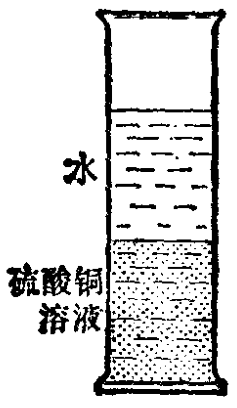
\includegraphics[width=3cm]{../pic/czwl2-ch5-1}
    \caption{}\label{fig:5-1}
\end{wrapfigure}

\xiaobiaoti{分子的运动}
组成物质的分子或原子(为了简单起见,以后我们只提分子)并不是静止不动的,而是在不停地运动着。
这可以从许多现象中看出来。
例如,一个空的瓶子(实际里边是空气)倒着放在装有红棕色二氧化氮气体的瓶子上,使两瓶口相对,
中间用玻璃片隔开,虽然二氧化氮比空气的密度大,但是当抽掉玻璃片以后,
可以看到红棕色的二氧化氮气体不断地向只有空气的瓶里运动,
最后两瓶气体的颜色变得完全相同,空气也运动到装二氧化氮的瓶里了。
这表明气体的分子是在不停地运动着。

象这样,不同的物质在互相接触时,彼此进入对方的现象叫做\textbf{扩散}。

扩散现象并不只是发生在气体之间,液体之间也有扩散现象。
在量筒里装半筒水,然后用长颈漏斗小心地把硫酸铜溶液倒进量筒的底部。
由于硫酸铜溶液比水的密度大,便沉在量筒的下部,和清水的界面非常清楚(图 \ref{fig:5-1})。
可是经过几天以后,蓝色的硫酸铜逐渐上升,界面变得模糊不清了。
再经过更长的时间,清水和硫酸铜溶液就混合均匀了。
这表明硫酸铜分子和水分子都在不停地运动。

固体之间也会发生扩散现象,只不过进行得很慢。
有人做过铅和金之间的扩散实验:将磨得很光滑的铅片和金片压在一起,
在室温下过了五年,结果铅片和金片便结合在一起了。
把它们切开后发现,铅和金相互渗透进去 1 毫米深。
可见,固体分子也在不停地运动。

大量实验表明,\CJKunderwave{一切物体里的分子都在不停地做无规则的运动}。

\begin{wrapfigure}{r}{4cm}
    \centering
    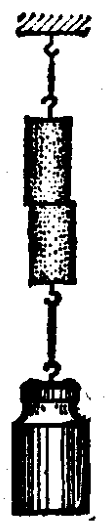
\includegraphics[width=1.5cm]{../pic/czwl2-ch5-2}
    \caption{分子引力实验}\label{fig:5-2}
\end{wrapfigure}

\xiaobiaoti{分子间的作用力}
既然物体是由分子组成的,而且分子在不停地运动着,那么,
为什么固体不会分散成一个一个的分子,而且能保持一定的体积和形状呢?
要把它的一部分跟另一部分分开,为什么比较困难呢?这是因为分子之间存在着引力的缘故。
当我们把物体的一部分跟另一部分分开时,就必须用力克服分子之间的引力。
把两块表面干净的铅压紧,由于分子间的引力,两块铅就结合在一起,
甚至在下面吊一个相当重的物体(图 \ref{fig:5-2}),也不能把它们拉开。

分子间还存在着互相排斥的力。这种斥力使分子间保持一定的间隙,而不是紧靠在一起。
固体和液体很难被压缩,就是由于分子间存在着斥力的缘故。

分子间的引力和斥力是同时存在的。
当分子间的引力和斥力相等时,分子处于平衡位置。
当分子间的距离十分靠近,小于平衡时的相互距离,斥力大于引力,分子间的作用力就表现为斥力。
当分子间的距离较大,大于平衡时的相互距离,引力大于斥力,分子间的作用力就表现为引力。
分子间的作用力随距离的增大而很快地减小。
当它们的距离大于分子直径的十倍以上时,分子间的作用力变得十分微弱,这时就常常近似地认为分子间没有作用力了。


\section{气体、液体和固体的分子结构}\label{sec:5-2}

我们知道,气体既没有一定的体积,又没有一定的形状;
液体有一定的体积,但没有一定的形状;
固体既有一定的体积,又有一定的形状。
气体、液体和固体的这种区别,可以用它们的分子结构的不同来说明。

\begin{wrapfigure}{r}{6cm}
    \centering
    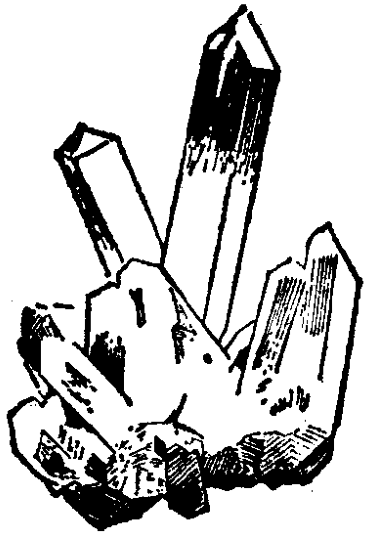
\includegraphics[width=5cm]{../pic/czwl2-ch5-3}
    \caption{水晶}\label{fig:5-3}
\end{wrapfigure}

\xiaobiaoti{气体}
气体很容易被压缩,说明气体分子间的距离比较大,在 0 ℃ 和 1 标准大气压下,
气体分子间的距离大约是分子直径的 10 倍。
这时分子间的作用力很小,可以近似地认为,气体分子除了相互碰撞或跟器壁碰撞外是不受作用力的。
所以,气体分子在没有跟别的分子或器壁碰撞时做匀速直线运动,只有受到碰撞时才改变速度的大小和方向。
由于气体分子的数目很大,分子间的相互碰撞十分频繁。整个看来,气体分子在做杂乱无章的运动。
由于气体分子可以在空间里到处移动,因此气体能充满它所能达到的空间,没有一定的体积,也没有一定的形状。

\xiaobiaoti{固体}
固体分子间的距离很小,只有几个埃,它们间的作用力很大,
绝大多数的分子只能在各自的平衡位置附近做无规则的振动。
正是由于这样,固体才能保持一定的体积和形状。

我们已经知道,固体分晶体和非晶体两类。
晶体的分子的排列是有规则的。因此晶体具有规则的天然形状。
图 \ref{fig:5-3} 是天然水晶的外形。
非晶体的分子的排列没有规则,因此非晶体没有规则的天然形状。

晶体又可分为单晶体和多晶体两类。
物体的分子按统一的规则排列成一个大晶体的,叫做单晶体。食盐、水晶等的单个晶体就是单晶体。
如果物体是由许多杂乱无章的小晶粒构成的,每个晶粒虽然有规则的外形,
但整个物体却没有规则的外形,这种晶体就叫做多晶体。常见的金属都是多晶体。

\xiaobiaoti{液体}
液体的分子结构介于气体和固体之间。
液变成气体时,体积增大一千倍左右,
变成固体时,体积变化不大,可见液体的分子结构比较接近于固体。

液体分子间的作用力比固体的小,分子的排列没有一定的规则,
液体分子也象固体分子那样在平衡位置附近做无规则的振动,
不过振动一段短时间后,就移动到别的位置,再振动一段时间后,又移动到别的位置。
正是由于液体分子运动的这个特点,使液体容易流动,没有一定的形状。
但液体分子间的距离也比较小,因此不易被压缩,而有一定的体积。

知道了气体、液体和固体的分子结构,就不难用分子运动论的知识来解释物态变化了。
例如,晶体的分子的排列是有规则的,在温度升高时,分子的振动加剧,
温度升高到一定程度,分子间的相互作用力已不能把分子限制在平衡位置附近振动,
于是有规则的排列被破坏,固体变为液体,这就是熔解。
不停地做无规则运动的液体分子中,总有一些分子的速度大到能够克服液面其他分子的吸引,
跑到液体外面去,成为气体分子,液体变为气体,这就是蒸发。


\lianxi

(1) 1 克蔗糖含有 $1.8 \times 10^{21}$ 个分子。把 1 克蔗糖放到蓄水 $10^{10} \lfm$ 的大水库中,
如果蔗糖分子均匀分布到整个水库中,每立方厘米的水中含有多少个蔗糖分子?

(2) 算算看,一个水分子的质量是多大?

(3) 撒一些粗盐块到一杯水里,过些时候,盐块看不见了,全杯水都变咸了。为什么?



\section{热能}\label{sec:5-3}

一切物体的分子都在不停地做无规则的运动。分子做无规则运动的快慢跟温度有关系。
把红墨水分别滴到热水和冷水中,可以看到,热水变色比冷水变色快。
在两种气体扩散的实验中,温度越高,两种气体扩散得就越快。
这些现象表明:温度越高,分子做无规则运动的速度就越大。
因为大量分子做无规则运动的速度跟温度有关,所以我们把物体里大量分子的无规则运动叫做\textbf{热运动}。

我们知道,在机械运动中,任何运动的物体都具有能,这种能叫做机械能。
在热运动中,任何运动的分子也具有能,物体中大量的做无规则运动的分子具有的能叫做\textbf{热能}。
机械能是能的一种形式,热能也是能的一种形式。

一个物体的温度升高,它的分子的运动加快,它的热能就增加;
    物体的温度降低,它的分子的运动变慢,它的热能就减少。


\section*{小实验}

倒一杯凉开水,把一块糖放到杯底。
然后用小勺取表面附近的水品尝,看看经过多长时间才能尝到有甜味。
取水时要小心,不要把水搅动。

再换用温开水来做这个实验,看看尝到表面附近的水有甜味经过的时间,
跟凉开水相比,是长了还是短了。

试解释你的实验结果。


\section{改变物体热能的方法}\label{sec:5-4}

用什么方法可以改变物体的热能呢?

用热传递的办法来改变物体的热能,这是大家都熟悉的。
在热传递的过程中,一个物体吸收了热量,温度升高,它的热能就增加。
反过来,         一个物体放出了热量,温度降低,它的热能就减少。

除了热传递,用做功的办法也可以改变物体的热能。

\begin{figure}[htbp]
    \centering
    \begin{minipage}{9cm}
    \centering
    \vspace{2cm}
    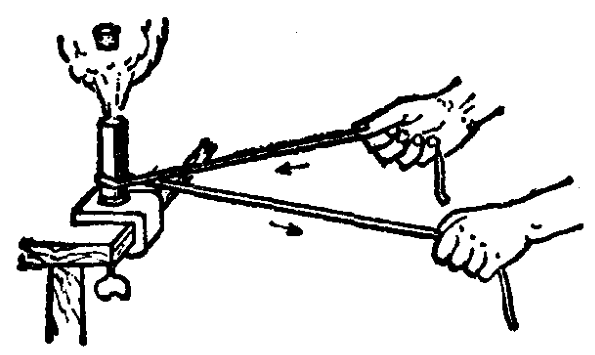
\includegraphics[width=8cm]{../pic/czwl2-ch5-4}
    \caption{克服摩擦做功使物体的热能增加}\label{fig:5-4}
    \end{minipage}
    \qquad
    \begin{minipage}{5cm}
    \centering
    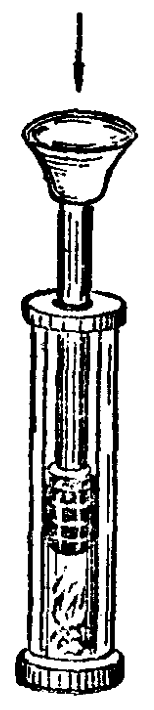
\includegraphics[width=1.5cm]{../pic/czwl2-ch5-5}
    \caption{压缩气体做功使物体的热能增加}\label{fig:5-5}
    \end{minipage}
\end{figure}

如图 \ref{fig:5-4} 所示,把一个薄壁金属管固定在支座上,管里装一些乙醚,然后用塞子塞紧。
把一根绳子缠在管子上,并迅速地来回拉绳子。过一会儿乙醚会沸腾,乙醚蒸气会把塞子冲开。
乙醚的温度升高,甚至达到了沸腾,说明它的热能增加了。
乙醚的热能增加,是因为克服绳子和管壁之间的摩擦做功而引起的。
我们通常说的摩擦生热,都是指的这类现象,即克服摩擦做功使物体的热能增加。

\begin{wrapfigure}{r}{6cm}
    \centering
    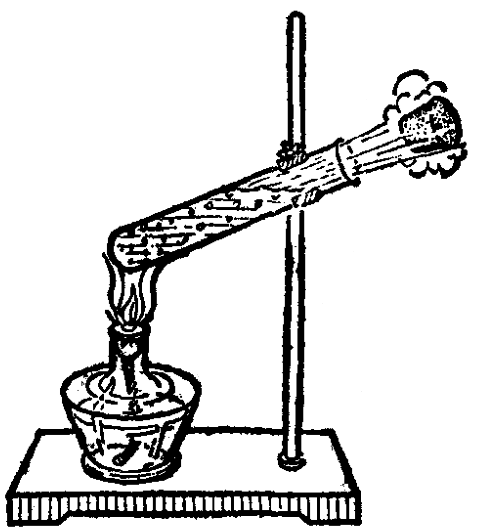
\includegraphics[width=5cm]{../pic/czwl2-ch5-6}
    \caption{气体膨胀做功使物体的热能减少}\label{fig:5-6}
\end{wrapfigure}

不但克服摩擦做功可以使物体的热能增加,用其他办法做功也可以。
如图 \ref{fig:5-5},在一个厚壁玻璃筒里放一块浸过乙醚的棉花,把活塞迅速地压下去,棉花就会燃烧。
这是因为压缩筒内空气做功,空气的热能增加,温度升高,达到了乙醚的着火点,浸了乙醚的棉花才燃烧起来。

上面讲的是,对物体做功,物体的热能就增加。
反过来,物体对外做功,热能就要减少。
也就是说,消耗热能也可以做功。
如图 \ref{fig:5-6} 所示,在试管里装一些水,用软木塞塞住。
加热使水沸腾,水蒸气会把软木塞冲开。水蒸气膨胀时对软木塞做功,消耗了水蒸气的热能。

可见,\CJKunderwave{改变物体热能的方法有两种:做功和热传递}。

一个温度升高了的物体,除非事先知道,我们将无法区别是由于做功还是由于热传递而使它的热能增加的。
例如一根锯条的温度升高了,我们将无法区别,是由于受到摩擦还是由于放在火上,而使它的热能增加的。
可见,做功和热传递对改变物体的热能是等效的。



\lianxi

(1) 举出几个用热传递的办法来改变物体热能的实例。

(2) 用锯锯木头,用锉锉铁块,过一会儿锯条或锉刀的温度会升高。为什么?

(3) 用打气筒给自行车车胎打气,过一会儿筒壁会热起来,这是为什么?

(4) 找一段粗金属丝,把它弄弯再弄直,这样反复数次后,用手摸一下弯折的地方,
你感到那里的温度发生了怎样的变化?解释这个现象。


\section{热功当量}\label{sec:5-5}

既然做功和热传递对改变物体的热能是等效的,那么功和热量之间是否有确定的数量关系呢?

最先研究这个关系的是英国物理学家焦耳。
他从十九世纪四十年代开始,花了大约四十年的时间,用各种不同的做功方法做了四百多次实验来研究这个关系。
以后又有许多人用更精确的方法来研究这个关系。
实验结果表明,功和热量之间存在着确定的数量关系:1 卡的热量跟 4.2 焦耳的功相当。
这个相当的关系在物理学上用
$$ 1\ka = 4.2 \jiaoer $$
来表示,它给出了热量的单位卡和功的单位焦耳之间的换算关系,叫做\textbf{热功当量}。

既然卡和焦耳这两个单位间存在确定的换算关系,就可以只保留一个,省去单位换算的麻烦;
现在的国际单位制正是这样。\CJKunderwave{国际单位制规定热量的单位跟功的单位一样,也是焦耳}。

焦耳不但是功和热量的单位,也是国际单位制中能量的单位。
各种形式的能,如机械能、热能、电能,单位都是焦耳。

热量的单位卡,是过去人们对功和热量相当的关系还不清楚的情况下规定的,现在已经可以废弃不用了。
不过因为卡这个单位长期沿用下来,要把以卡为单位的许许多多技术资料都改成以焦耳为单位,还需要一段时间。

\section*{阅读材料}

\begin{wrapfigure}[14]{r}{6cm}
    \centering
    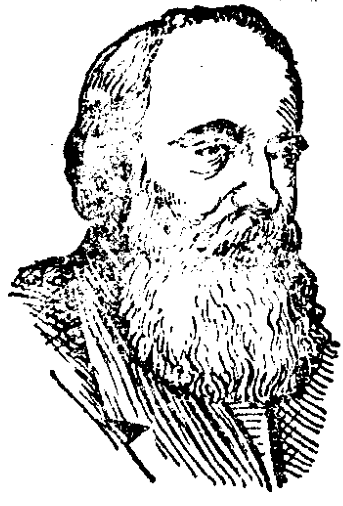
\includegraphics[width=5cm]{../pic/czwl2-ch5-joule}
    \caption*{焦耳(1818~1889)}\label{fig:5-joule}
\end{wrapfigure}

焦耳是英国物理学家。焦耳没有上过学,他的科学知识几乎全是靠自学获得的。
1840 年,他多次做了导体通过电流发热的实验。
根据实验结果,写出了他的第一篇科学论文《电流析热》,提出了电能转化为热能的规律。
这时焦耳才二十二岁。这个规律就是我们将在第九章学到的焦耳定律。

焦耳探讨了各种形式能的转化关系。1843 年 8 月,他在英国学术协会上作了《论电磁热效应和热功当量》的报告。
报告的结论是:自然界的能量是不能消灭的,消耗了机械能,总能得到相当的热能。

焦耳采用自己精心设计的量热器,测定了热量和功的数量关系,即热功当量。
焦耳的实验结果已经相当精确了,但是他不满足已有的成就,不断改进方法,继续进行实验,
从十九世纪四十年代开始到七十年代近四十年当中,用各种方法进行了四百多次实验。
他得到的热功当量的数值,保持了三十年没有较大的变化,这在物理学史上是极为罕见的。



\section{能的转化和守恒定律}\label{sec:5-6}

现在我们从能的转化的角度来探讨一下改变物体热能的两种方法。

用热传递的方法来改变物体的热能,实际上是热能从一个物体转移到另一个物体的过程。
参加热传递的两个温度不同的物体,一个放出热量,另一个吸收热量。
一个放出多少热量,它的热能就减少多少。
另一个吸收多少热量,它的热能就增加多少。
我们知道,如果这两个物体都没有从别的物体那里吸收热量,也没有把热量传递给别的物体,
那么一个放出的热量跟另一个吸收的热量总是相等的。
可见一个物体减小多少热能,另一个就增加多少热能。
热能从一个物体转移到另一个物体,是既不增加,也不减少,而保持守恒。

用做功的方法来改变物体的热能,实际上是热能和其他形式的能相互转化的过程。
克服摩擦做功或者压缩气体做功而使物体的热能增加,要消耗机械能,这时机械能转化为热能。
而且做多少功,即消耗多少机械能,就得到多少热能。
气体膨胀做功而使物体的热减少,这时热能转化为机械能,而且做多少功,即消多少热能,就得到多少机械能。
可见,在热能和机械能相互转化的过程中,能量同样是既不增加,也不减少,而保持守恒。

除机械能、热能外,还有其他形式的能,如电能、光能、原子能、化学能等等。
各种形式的能都可以在一定条件下相互转化。
水轮机带动发电机发电,机械能转化为电能;
电动机带动水泵把水抽到高处,电能又转化为机械能。
木柴燃烧发出热和光,化学能转化为热能和光能;
植物吸收太阳光进行光合作用,光能又转化为化学能。
大量的实验事实告诉我们,任何一种形式的能在转化成其他形式的能的过程中,总的能量都是守恒的。

所以,\textbf{能量既不会消灭,也不会创生,它只会从一种形式转化成另一种形式,
或者从一个物体转移到另一个物体,而能的总量保持不变}。这个规律叫做\textbf{能的转化和守恒定律}。

能的转化和守恒定律,是自然界最普遍、最重要的基本定律之一,是我们认识自然和改造自然的重要科学依据。


\section{能源的开发和利用}\label{sec:5-7}

机器的运转,汽车的行驶,火车的开动,飞机的飞行……都要消耗一定的能量。
就是做饭、照明、取暖等日常生活也都要消耗能量。凡是能够提供能量的东西都可以叫做能源。
煤、石油和天然气在燃烧时放出大量的热能,它们就是能源。
流动的水和空气可以推动水轮机和风力发动机工作,它们也是能源。

\begin{figure}[htbp]
    \centering
    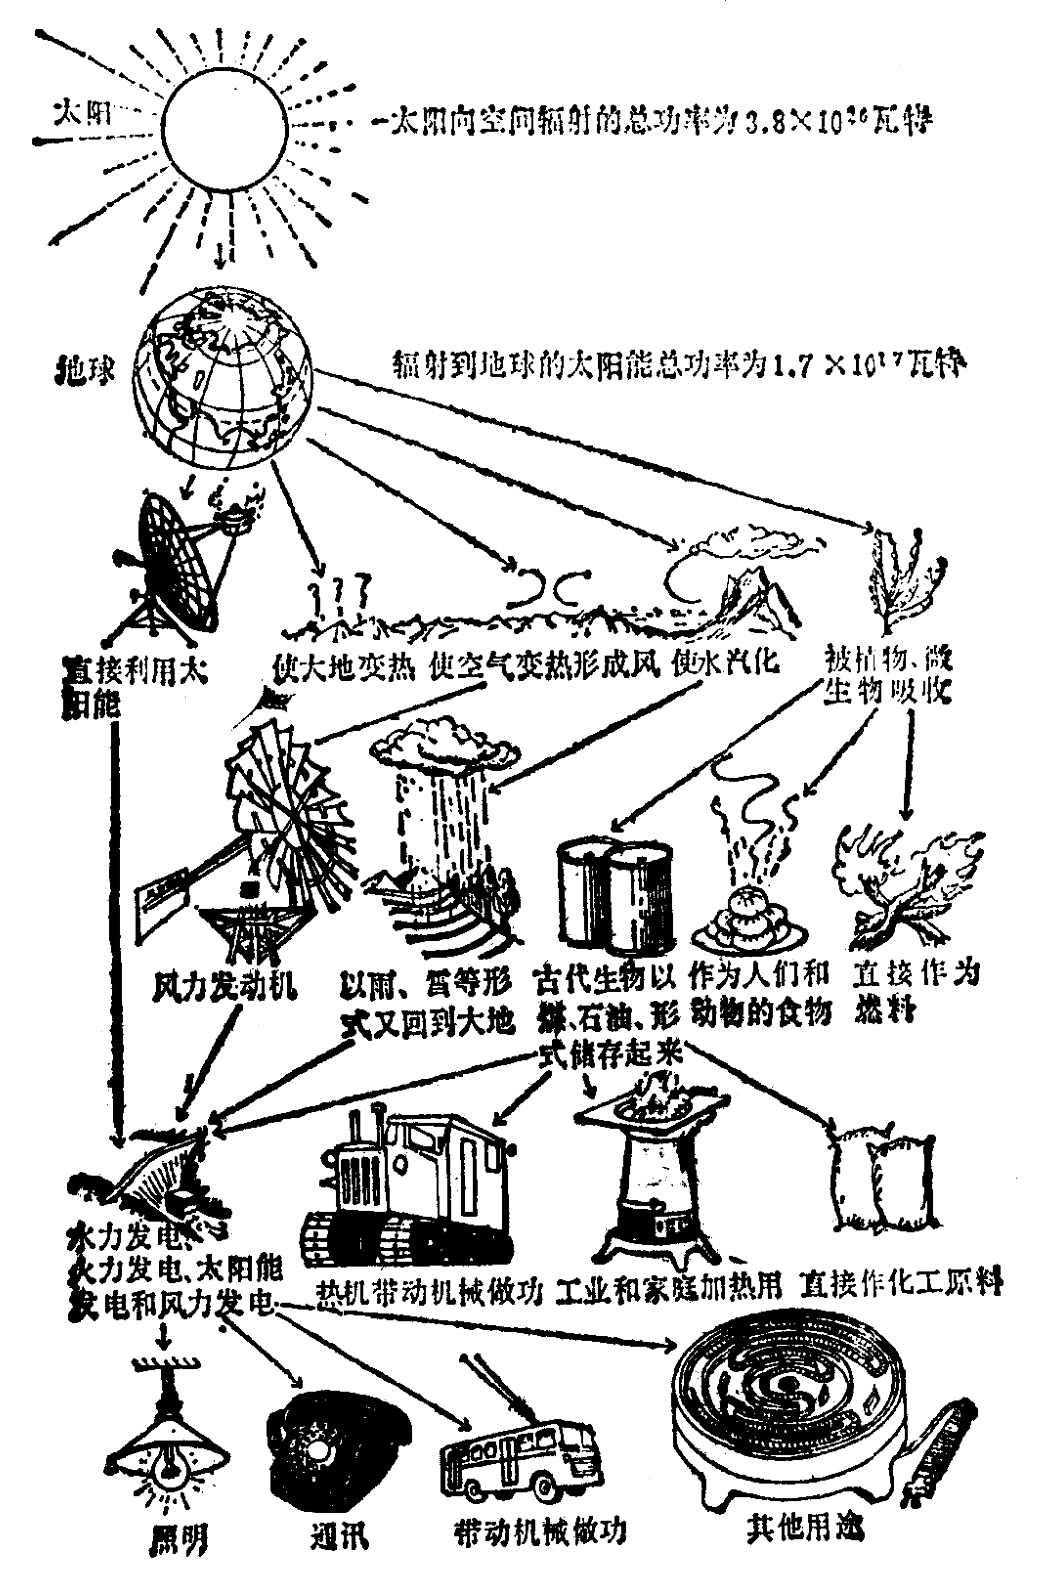
\includegraphics[width=0.7\textwidth]{../pic/czwl2-ch5-7}
    \caption{太阳能的利用示意图}\label{fig:5-7}
\end{figure}

随着科学技术的发展,人类开发和利用能源的范围不断扩大。
但是,到目前为止,人类社会使用的仍然主要是煤、石油和天然气。
现代的生产和生活中能量的消耗愈来愈大,近些年来更有急剧上升的趋势。
煤、石油和天然气等的贮量总是有限的,不可能无限制地满足人们不断增长的需要。
这就是近年来人们常常谈到的能源危机。为了解决这个问题,我们要不断地探索能的转化的新途径,
有效地利用已经探明的能源,努力开发和利用新的能源。

新的能源中,当前人们最为瞩目的是原子能。
原子核发生变化时释放的能量叫做原子能,也叫核能。
人们对原子能的利用从四十年代开始到现在已经有了巨大的发展,已经可以建立核电站生产大量的电能。
目前,我国也正在筹建功率很大的核电站。

太阳发出的光和热具有能,它是一个十分巨大的天然能源。
据计算,到达地面的太阳能的总量大约是地球上目前正在为人类利用的各种能源的总功率的一、两万倍。

人类利用煤、石油和天然气的能量,利用水能和风能,归根到底都是间接利用太阳能,
因为它们都是来源于太阳的光和热(图 \ref{fig:5-7})。
直接利用太阳能的比较简便的方法是把太阳能转化为热能,如在第一章介绍的太阳灶和太阳炉。
在温度要求不太高的情况下,还可以采用吸热式集热箱来获得太阳能。
集热箱实际上是一个开有透明窗口、内壁涂黑的保温箱。
保温箱的构造如图 \ref{fig:5-8} 所示,在太阳照射下,箱内的温度可以超过一百度。
(这种集热箱能够使箱内温度升高的道理,可以根据你学过的热学知识来解释。)
利用太阳能获得的热能,可以用来产生水蒸气(或热气),再利用水蒸气(或热气)膨胀带动机器作功,
如带动水泵的太阳能水泵,带动汽轮发电机组的太阳能发电。
还可以直接利用太阳能发电,第七章介绍的硅光电池,就是直接利用太阳能获得电能的。

\begin{figure}[htbp]
    \centering
    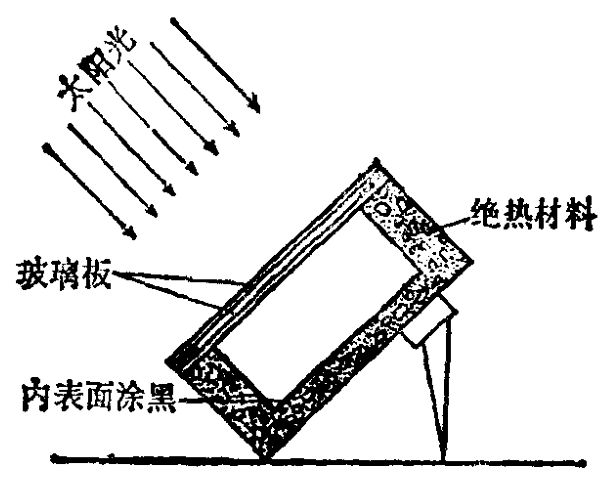
\includegraphics[width=0.4\textwidth]{../pic/czwl2-ch5-8}
    \caption{}\label{fig:5-8}
\end{figure}

太阳能具有取之不尽、用之不竭、清洁无污染等优点。
因此,太阳能的利用引起了各国的重视,有着广阔的发展前途。
可以预料,到二十一世纪,太阳能将是人们利用的主要能源之一。

我国是能源比较丰富的国家。已经探明,我国煤的储藏量达 6000 亿吨,居世界第三位,
石油的储藏量居世界第八位,核能原料也十分丰富。
解放以来我国能源开发的增长速度是比较快的。
解放后三十年,全国能源生产总量增长了 26 倍。
但是,随着现代化建设的发展和人民生活水平的提高,对能源的需要也将不断增长。
因此,我国也在大力研究能源的合理开发问题。

为了适应现代化建设对能源的需要,在抓好能源开发的同时,还必须注意能源节约。
目前我国在能源的生产、运输、转化、使用等方面都存在很大浪费,主要原因有技术陈旧、设备落后、管理不善等。
为了节能,需要采取多种措施,例如,采取先进的能耗小的工艺流程,进行以节能为中心的技术改造,
以省煤、省油、效率高的锅炉、热机、电机等设备替换陈旧落后的设备,规定各种产品和用能设备的能耗标准,
制定能源使用中的奖惩制度,等等。
我们每个同学,不但自己要注意节能,还应该注意宣传节能的意义,这也是对祖国社会主义现代化建设的贡献。


\lianxi

(1) 1 焦耳的热能,可以使 10 克水的温度升高多少度?

(2) 一壶 5 千克的水,温度从 20 ℃ 升高到 100 ℃,吸收的热量是多少卡?相当于多少焦耳?

用这些功来把你举高,可以把你举多高?

(3) 1 千克汽油完全燃烧放出的热量是多少焦耳?

(4) 举几个常见的热能和机械能相互转化的例子。


\section*{复习题}

(1) 什么现象表明物体的分子在不停地做无规则的运动?
为什么把物体里大量分子的这种无规则运动叫做热运动?

(2) 物体里分子间的作用,在什么情况下表现出斥力?
在什么情况下表现出引力?在什么情况下可以认为没有作用力?

(3) 气体、液体和固体三者之间的主要差别是什么?怎样用物质的分子结构来说明这种差别?
在气体、液体和固体这三种状态中,物质究竟以哪种状态存在是由什么来决定的?

(4) 什么叫做热能?改变物体的热能有哪两种方法?

(5) 热功当量表示的是什么关系?写出焦耳和卡这两种单位的换算关系。

(6) 什么是能的转化和守恒定律?



